\chapter{Rnw example chapter}
\label{chap:rnw}





This document was generated on Wed Apr 13 15:53:04 2016.

As shown in Figure \ref{fig:some_fig} and in Table \ref{tab:rtab1} we can see that bla bla.


\begin{knitrout}
\definecolor{shadecolor}{rgb}{0.969, 0.969, 0.969}\color{fgcolor}\begin{figure}
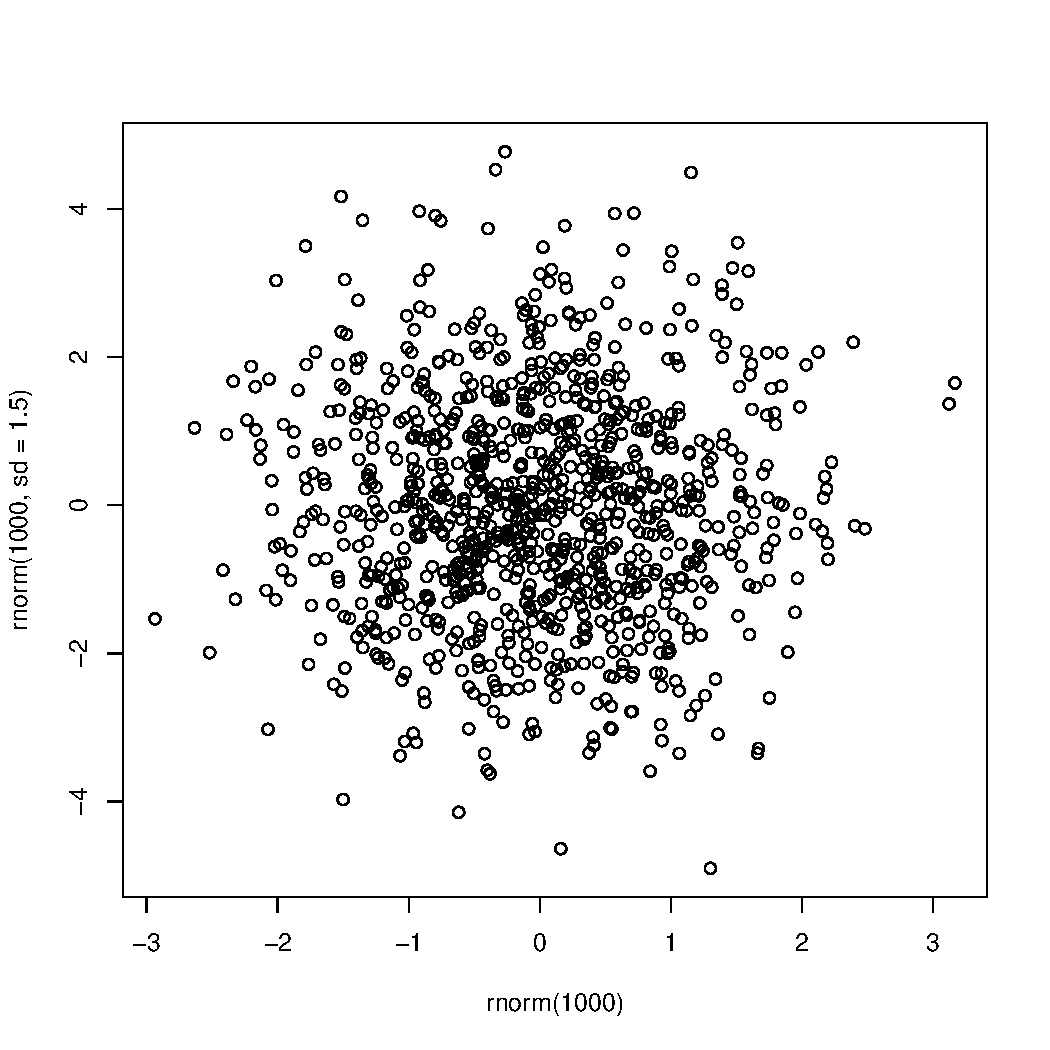
\includegraphics[width=\maxwidth]{figure/some_fig-1} \caption[{\bf Figure title } Rest of description]{{\bf Figure title } Rest of description}\label{fig:some_fig}
\end{figure}


\end{knitrout}






% latex table generated in R 3.3.0 by xtable 1.8-2 package
% Wed Apr 13 15:53:04 2016
\begin{table}[ht]
\centering
\begin{tabular}{rr}
  \hline
A & B \\ 
  \hline
  1 & -0.63 \\ 
    2 & -0.67 \\ 
    3 & 0.06 \\ 
    4 & -0.38 \\ 
    5 & -0.22 \\ 
    6 & 0.95 \\ 
    7 & 1.83 \\ 
    8 & 0.24 \\ 
    9 & 1.16 \\ 
   10 & 1.34 \\ 
   \hline
\end{tabular}
\caption{\bf{ Table title } Table description} 
\label{tab:rtab1}
\end{table}

